
In this section we provide a brief summary of the theory of
gravitational lens time delays. We have distilled much of this from the
excellent exposition of Schneider and Kochanek \citep{SKW06}, as well as
the various key papers we cite.

% Lensing, Fermat's principle and potential. Time delay surface.

Fermat's Principle of Least Time holds for the propagation of light rays
through curved spacetime. The light travel time through an isolated, thin
gravitational lens is given by
\begin{align}
    \tau(\x) &= \frac{\Ddt}{c} \cdot \Phi(\x,\y), \\
    \text{where\;\;} \Phi(\x) &= \frac{1}{2}\left(\x - \y\right)^2 - \psi(\x).
\end{align}
Here, $\x$ denotes the light source's apparent position on the sky, and
$\y$ is the position of the unlensed source. The difference between the
observable position~$\x$ and the unobservable position~$\y$ is the
scaled deflection angle~$\deflectionangle({\x})$, which is typically
$\sim1$~arcsecond in a galaxy-scale strong gravitational lens system.
$\psi(\x)$ is the scaled gravitational potential of the lensing object,
projected onto the lens plane. Both $\deflectionangle(\x)$ and $\psi(\x)$ can be
predicted given a model for the mass distribution of the lens.

Images form at the extrema of the light travel time, where $\grad
\tau(\x) = \grad \Phi(\x) = 0$ \citep{Schneider1985}. For this reason,
$\Phi(\x)$ is known as the ``Fermat potential.'' This quantity can also
be thought of as the spatially-varying refractive index of the lens. The
arrival time itself is not observable, but differences in arrival time
between multiple images are. In the above approximation, the  ``time delay'' $\Delta \tau_{\rm AB}$
between image A and
image B can be predicted via
\begin{equation}
    \Delta \tau_{\rm AB} = \frac{\Ddt}{c} \Delta \Phi_{\rm AB} \label{eq:timedelay}
\end{equation}
where $\Delta \Phi_{\rm AB}$ is the Fermat potential difference between the
two image positions.
Figure~\ref{fig:lineofsightcartoon} illustrates the origin of the
time delay between the images in a gravitational lens system. The small
magnitude of the fractional time delay (typically $\Delta\tau \sim 10$~days out of
$\Ddt/c \sim 10^{12}$ days light travel time)
is commensurate with the square of the
deflection angle (typically $|\deflectionangle|\sim1$~arcsecond, or $\sim 5\times10^{-6}$
radians).

\begin{figure*}
\centering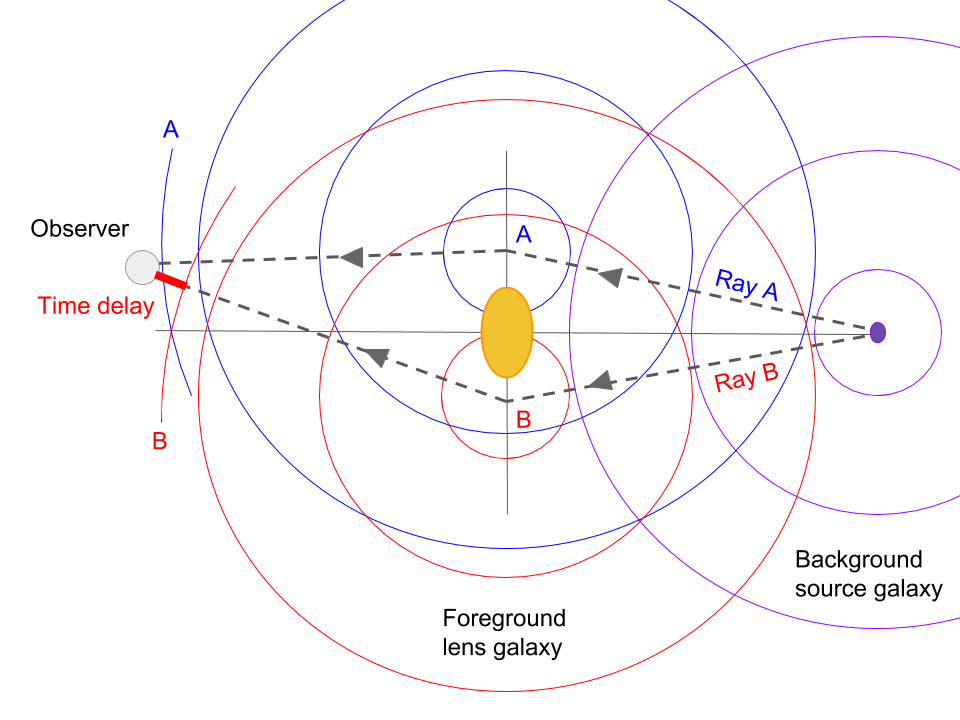
\includegraphics[width=0.96\textwidth]{figures/wavefront-schematic.png}
\caption{Schematic diagram, adapted from \citep{TreuAndEllis2015},
illustrating the origin of the gravitational time delay.}
\label{fig:lineofsightcartoon}
\end{figure*}

% Time delay distance.

We see from Equation~\ref{eq:timedelay} that given a mass
model that predicts $\Delta \Phi_{\rm AB}$, we can infer the ``time
delay distance'' $\Ddt$ from a measured time delay $\Delta \tau_{\rm AB}^{\rm obs}$.
This distance is actually a combination of angular diameter
distances:\footnote{As \citet{SKW06} point out, $\Ddt$ can be written more simply in terms
of comoving angular diameter distances, but most of the literature uses the
formula in Equation~\ref{eq:ddt}.}
\begin{equation}
    \Ddt = (1+\zd) \frac{\Dd \Ds}{\Dds}  \label{eq:ddt}
\end{equation}
These angular diameter distances can be predicted given the redshifts
of the lens and source, $\zd$ and $\zs$, and an assumed world model with
cosmological parameters~$\cospars$.

% Importance of mass distribution in lens.

Knowledge of the lens mass distribution is of critical importance to the
success of this cosmological inference


Sensitivity analysis in \citep{SKW06}.

% Model (mass-sheet) degeneracy and its generalizations

Model assumptions. Flexible models degenerate under the mass sheet transformation.
Degeneracy between model parameters. Break with more information: strong assumptions about parameterized forms?
Auxiliary information about the model?

% Importance of mass along the line sight - the universe is not Friedmann Lemaitre Robertson Walker.

Simple line of sight effects following \citep{SKW06}. External convergence and shear.
Multi-plane formalism.

\begin{figure*}
% \centering\includegraphics[width=0.96\textwidth]{figures/line-of-sight-cartoon.pdf}
\caption{Cartoon illustration of line of sight effects in time delay
lens cosmography. Structures both within and outside the main lens
plane provide weak deflections to the light rays, affecting both the
image positions and time delays.} \label{fig:lineofsightcartoon}
\end{figure*}
